% !TEX root = main.tex
%%%%%%%%%%%%%%%%%%%%%%%%%%%%%%%%%%%%%%%%
%%%%%%%%%%%%%%%%%%%%%%%%%%%%%%%%%%%%%%%%
\section{\approach} \label{sec:t5}
%%%%%%%%%%%%%%%%%%%%%%%%%%%%%%%%%%%%%%%%
%%%%%%%%%%%%%%%%%%%%%%%%%%%%%%%%%%%%%%%%

\subsection{Learning to Generate Complete Log Statements}

\subsubsection{Text-to-Text-Transfer-Transformer (T5)}


The T5 model was introduced by Raffel \etal \cite{raffel2019exploring} to support multitask learning in the domain of NLP (Natural Language Processing). The novel idea behind the T5 model is to reframe NLP tasks in a unified text-to-text format in which the input and output are always text strings. For instance, a single model can be trained to translate across languages  (\eg learning the translation of sentences from English to French) and to autocomplete sentences. This approach is based on two phases: \textit{pre-training}, which allows defining a shared knowledge-base useful for a large class of sequence-to-sequence tasks, and \textit{fine-tuning}, which specializes the model to specific tasks of interest. 

\subsubsection{A peek under the hood}
T5 is based on the transformer model architecture that allows handling a variable-sized input using stacks of self-attention layers. When an input sequence is provided, it is mapped into a sequence of embeddings passed into the encoder. The T5, in particular, and a transformer model \cite{vaswani2017attention}, in general, offer two main advantages over other state-of-the-art models: (i) it is more efficient than RNNs since it allows to compute the output layers in parallel, and (ii) it is able to detect hidden and long-ranged dependencies among tokens, without assuming that nearest tokens are more related than distant ones. The latter, is particularly relevant in code-related tasks since a variable declaration may be distant from its usage. To this extent, the T5 model can relate the tokens representing the declaration of a local variable in the first statement of a method with the tokens implementing a return statement in which the value of such a variable is returned (despite the fact that the two statements could be far apart). 

In our work, we rely on the same T5 architecture (\ie T5$_{small}$) that has been exploit by Mastropaolo \etal \cite{mastropaolo2022using} to support the task of complete log statements generation. In this regard, the authors relied on such T5 variation because it allowed a reasonable trade-off between the training time needed to train a  60M parameters model (\ie T5$_{small}$)  and the results they were able to achieve.
 
Specifically, the T5\textsubscript{\textit{small}} architecture is characterized by six blocks for encoders and decoders. The feed-forward networks in each block consist of a dense layer with an output dimensionality ($d_{ff}$) of 2,048. The \textit{key} and \textit{value} matrices of all attention mechanisms have an inner dimensionality ($d_{kv}$) of 64, and all attention mechanisms have eight heads. All the other sub-layers and embeddings have a dimensionality ($d_{model}$) of 512. The code implementing the T5 model is publicly available in our replication package \cite{replication}.


\subsubsection{Pre-training Dataset}

To build the dataset, we used GHS (GitHub Search) the search tool by Dabic \emph{et al.} \cite{dabic2021sampling} that allows using tailored specifications to identify Github \cite{github} projects. Specifically, we used the same selection criteria used by Mastropaolo \etal \cite{mastropaolo2022using} in the work presenting LANCE.
In this regard, we selected all public non-forked \java projects with minimum 500 commits, 10 contributors, and 10 stars.
The selection criteria on the number of commits, contributors, and stars are necessary to avoid personal/toy projects, and 
by choosing non-forked repositories we reduced the chances to mine duplicated code. 
We collected 6,352 candidate projects of which we were able to clone the latest snapshot of 3,865 of them. 
We scanned all the cloned repositories to assess if a \texttt{POM} (Project Object Model)\footnote{A POM file is used in Maven to declare dependencies towards Maven libraries.} file or a \texttt{build.gradle}\footnote{A build.gradle file describes the build configuration, tasks, plugins and dependencies for a gradle project.} file was present in the projects' directory.
All the projects using a different build automation tool were discarded.
Whilst Mastropaolo \etal \cite{mastropaolo2022using} mined only Maven projects, we also decided to expand our search to Gradle projects. Such a design choice would likely increase the chances of identifying new relevant data points.
To have an even more cohesive codebase we required the projects to have an explicit dependency on either Apache Log4J \cite{log4j}, a well known Java logging library, or on SLF4J (Simple Logging Facade for Java) \cite{slf4j}, an abstraction for Java logging frameworks similar to Log4J.
We found out that 2,978 of the cloned repositories had an explicit dependency on either Log4J or SLF4J. Afterwards, we leveraged srcML \cite{srcml} to extract all the \java methods from the selected projects. In details, we used the \java methods srcML representation to automatically remove all the inline comments, and to identify all the methods' log statements. We then filtered out all methods containing log statements with custom log levels (\emph{i.e.}, log levels different from \texttt{FATAL}, \texttt{ERROR}, \texttt{WARN}, \texttt{DEBUG}, \texttt{INFO}, and \texttt{TRACE}).
The purpose of this filtering was to remove all methods containing log statements with project ad-hoc log levels, thus that are not generalizable.
Then, we used \emph{javalang} \cite{javalang} to tokenize the methods obtaining the method representation as a flat stream of tokens.
Once we had the tokenized Java methods, we removed all the instances having $\#tokens < 10$ or $\#tokens \geq 512$, similar filtering has been done in previous works \cite{mastropaolo2021empirical,tufano2021automating,tufano2022using,ciniselli2021empirical, Tufano:tosem2019} to limit the computational expenses of training DL-based models.
To avoid methods overlapping between training, validation, and test datasets we also removed all the duplicates. 
Finally, we filtered out all the methods containing non-English characters to obtain an even more coherent codebase. 
To ensure the quality of the processed dataset we performed a manual analysis on a sample of 200 random methods. 
The purpose of such an analysis was threefold: (i) ensure  the dataset did not contain false-negative logs (\emph{i.e.}, log statements not identified during the creation of the dataset) (ii) ensure the dataset did not contain false-positive logs (\emph{i.e.}, pieces of code wrongly identified as log statements), and (iii), guarantee that all the instances were preprocessed correctly.
This left us with a dataset of 12,917,300 \java methods of which 244,588 contain at least one log statement. We used the dataset to build the pre-training and fine-tuning datasets summarized in \tabref{tab:ds-summary-1}. 

\begin{table*}[h]
	\centering
	\caption{Num. of methods in the datasets used in the differentiated replication of LANCE}
		\label{tab:ds-summary-1}
	\begin{tabular}{ccccccccc}
		\hline
		\multirow{2}{*}{\textit{\textbf{Dataset}}} & \multicolumn{2}{c}{\textbf{train}} & \textbf{} & \textbf{eval} & \textbf{} & \textbf{test}  \\ \cline{2-3} \cline{5-5} \cline{7-7} 
		& \textbf{w/ log} & \textbf{w/o log} & \textbf{} & \textbf{w/ log} & \textbf{} & \textbf{w/ log} \\ \hline
		\textit{Pre-training dataset}              & -               &      12,671,475  &           & -               &           &  -               \\
		\textit{Single-log fine-tuning dataset}               & 229,703         & -                &           & 28,763          &           & 28,698          \\
		\textit{Multi-log fine-tuning dataset}               & 192,773         & -                &           & 24,092         &           & 24,088          \\ \hline
		\textit{Single-log Context-Aware fine-tuning dataset}               & 229,703         & -                &           & 28,763          &           & 28,698          \\
		\textit{Multi-log Context-Aware fine-tuning dataset}               & 192,773         & -                &           & 24,092         &           & 24,088          \\ \hline
	\end{tabular}
\end{table*}



\begin{figure}[h!]
	\label{fig:pre-training}
	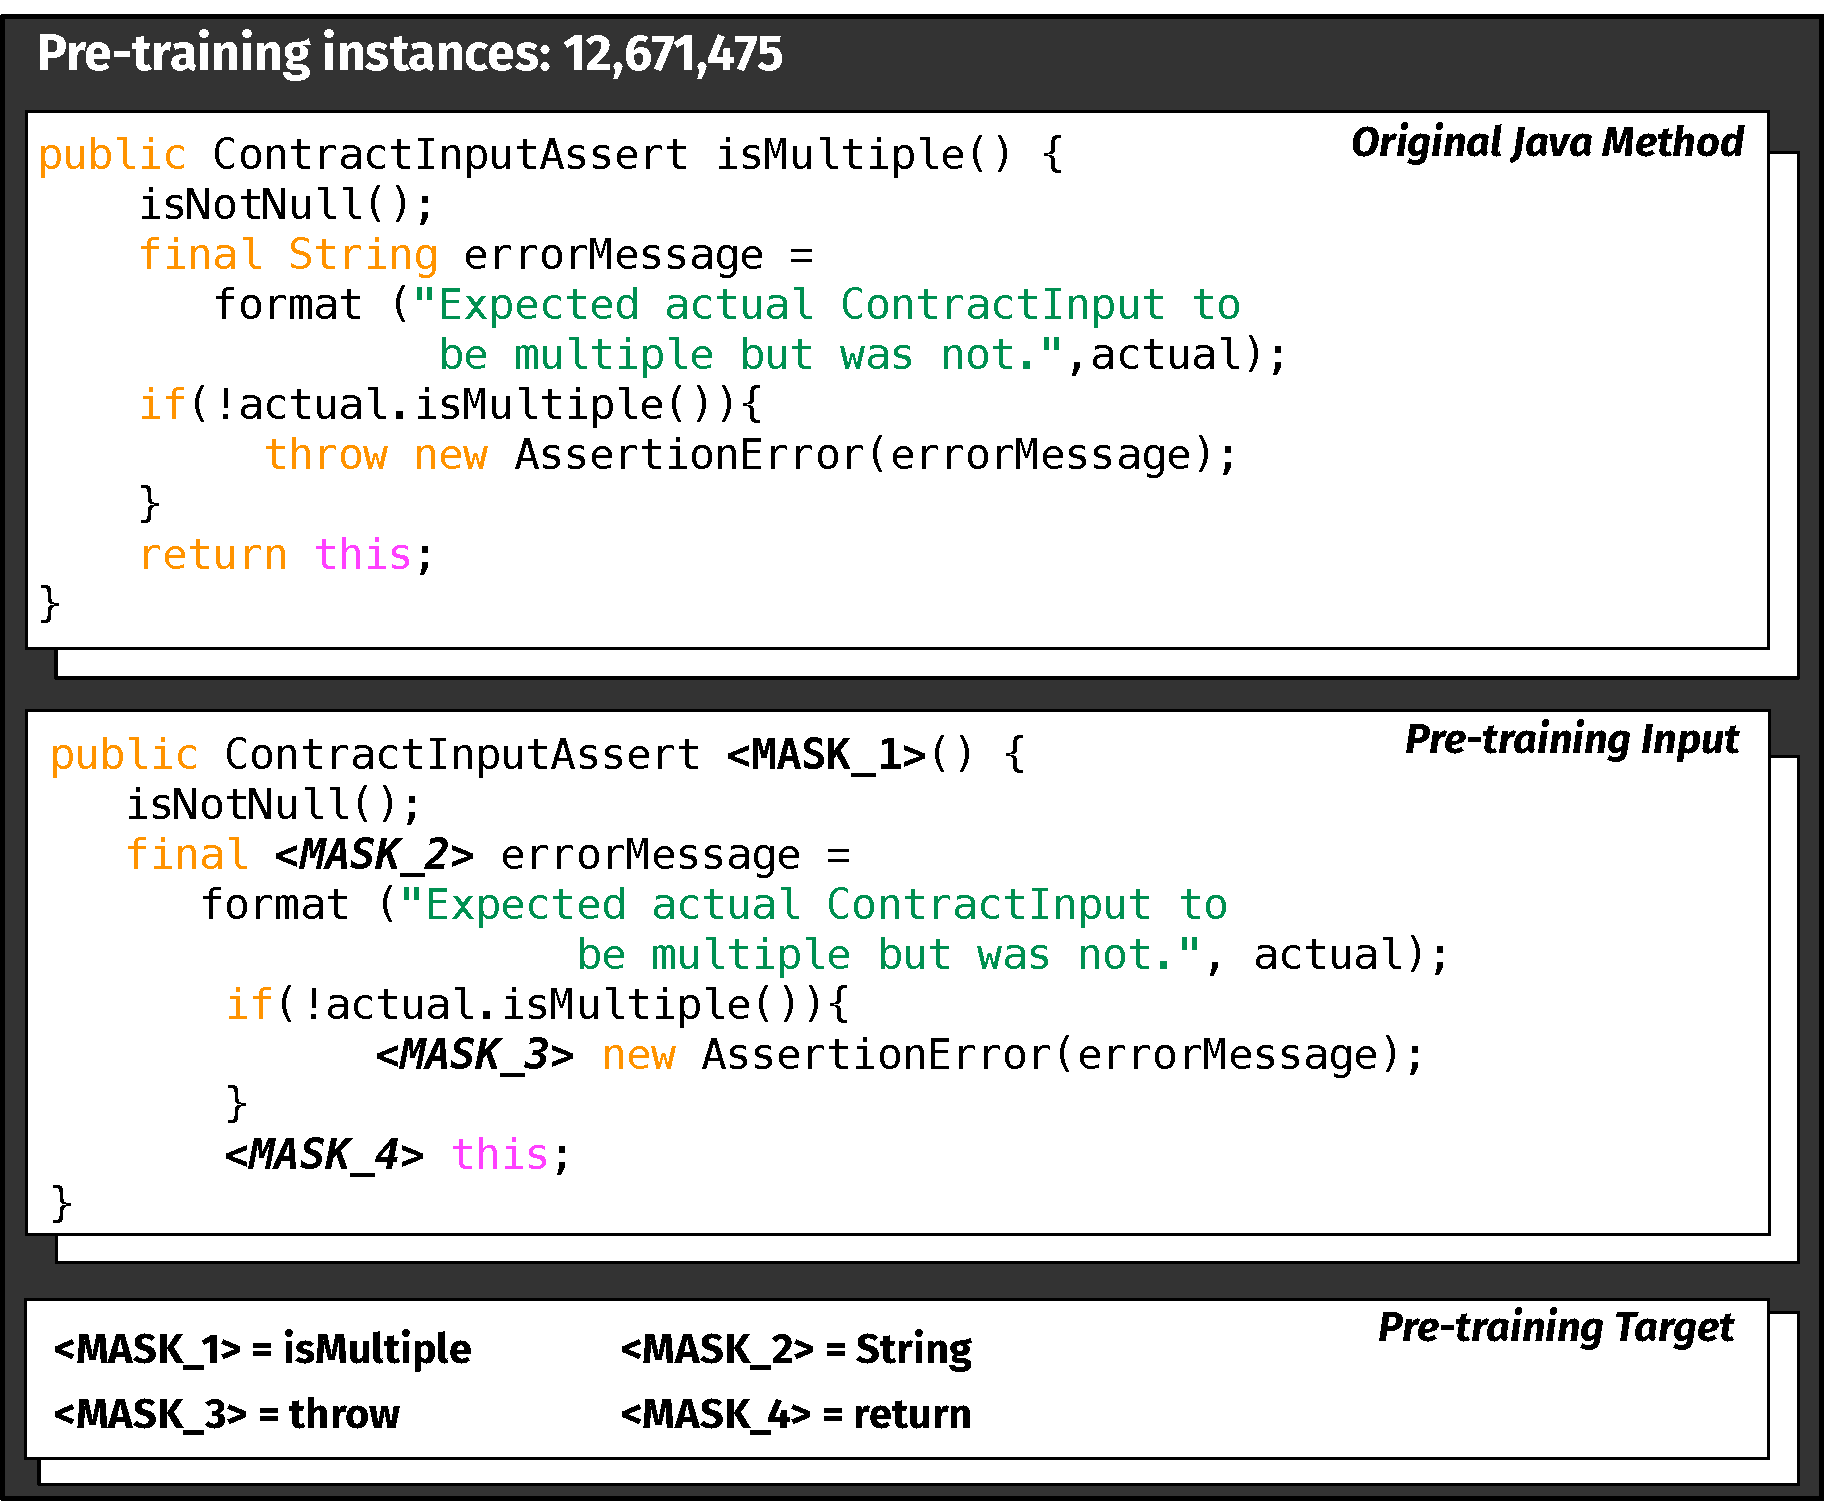
\includegraphics[width=\columnwidth]{img/pre-training.pdf}
		\caption{Example of T5 Pre-training instance.}
\end{figure}




\subsubsection{Single-Log fine-tuning dataset} \label{sec:single-log-dataset}
To build the fine-tuning dataset that replicate what have been done by Mastropaolo \etal \cite{mastropaolo2022using}, we pre-process each training instance (\ie \java method in the training-set) by removing one log statement at a time from the \java method. This process, leaves us with a pair $\langle M_i, M_t \rangle$ featured by the input and the target sequence in which $M_i$ represents the original \java method $M$ without the target log statement, while $M_t$ is the original \emph{Java} method equivalent to $M$. For those methods containing more than one log statement, we created $n$ pairs of input-target sequences, with $n$ being the number of log statements in the method. To ensure that after the log statement removal all the instances are still valid Java methods, we parsed each instance we created using JavaParser \cite{javaparser} and removed all the instances the tool was not able to parse or instances that after the instrumentation have been duplicated. Finally, the fine-tuning dataset replicating the approach implemented by Mastropaolo \etal \cite{mastropaolo2022using}, has been split into 80\% training, 10\% validation, and 10\% test (see \tabref{tab:ds-summary-1}). 
While the instances featuring the test set have been used to assess the performance of our model (\emph{i.e.}, its ability to generate complete log statements and inject them in the correct location), the validation set was used to find the best configuration of hyperparameters (\secref{sec:training}). Later, we used the validation dataset also to perform early-stopping taming the over-fitting problem.

We use such a dataset to replicate LANCE on a more extensive and curated set of instances.
Nonetheless, even when considering that LANCE represents a concrete step ahead in automating logging activities, the limiting factor affecting the generation of meaningful log messages would pose questions about the usefulness of such an approach.  

In this regard, we made a first step toward tackling this limitation by combining LANCE with Information Retrieval.
As introduced in \secref{sec:intro}, the main idea is to augment the input of a given \java method $M_{j}$ with log messages belonging to the most similar methods featured within the newly curated training set. In detail, we build the new  \textcolor{blue}{log message context-aware} dataset starting from the xxxx instances provided in the \textit{Single-log fine-tuning dataset}. In doing so, from a Java method $M_{tr_j}$ in the original training set (\tabref{tab:ds-summary-1}), we strip away all the log statements in it, obtaining a new log-free version $M_{tr_j}^{1}$ in which no log statements are found. Then, the  same procedure is performed to the remaining methods featuring the training, test and eval set. Later, we compute the $K$ most similar log-free methods using the \textit{Jaccard Similarity \cite{hancock2004jaccard}} for each set (\ie, training, eval and test).

\begin{equation}
	J(M_{tr_i}^{1}, M_{tr_j}^{1})=\frac{|M_{tr_i}^{1}  \cap M_{tr_j}^{1} |}{|M_{tr_i}^{1}  \cup M_{tr_j}^{1} |}
\end{equation}

\begin{equation}
	J(M_{test_i}^{1}, M_{tr_j}^{1})=\frac{|M_{test_i}^{1}  \cap M_{tr_j}^{1} |}{| M_{test_i}^{1}  \cup M_{tr_j}^{1} |}
\end{equation}


\begin{equation}
	J(M_{eval_i}^{1}, M_{tr_j}^{1})=\frac{|M_{eval_i}^{1} \cap M_{tr_j}^{1} |}{| M_{eval_i}^{1} \cup M_{tr_j}^{1} |}
\end{equation}

To compute such a metric, for each pair $\langle M_{Z_i}^{1}, M_{tr_j}^{1} \rangle$ with $Z \in \{ training, eval, test\}$ we create a set of the \java tokens featuring of the methods, ending up with an unique list of \java tokens (\ie each token appears only once in such list) for both methods.
Finally, we use the \textit{Jaccard Similarity} score to rank the most similar $K=\{1,3,5\}$ methods to $M_{Z_i}^{1}$, from which we retrieve all the log messages accompanying the log statements in the $K$ retrieved methods.

From the moment that among the $K$ most similar methods, we might find log statements having the same log message, we disentangle such a case by adding to each retrieved log message the \textit{Jaccard Similarity} score of the log message that has been retrieved from the method $M_{tr_j}^{1}$ sharing the highest number of tokens with $M_{Z_i}^{1}$.

As for those instances where the log statements (by construction) do not include log messages, the augmentation process returns as output the original input sequence (\ie \java method with a stripped log statement) taken as input.


\figref{} shows an example of augmented Java method from log message context-aware dataset.


%As described in \secref{sec:intro}, our multi-log injection approach is built on top of two separate models: (i) a classification model that predict whether a method requires or not log statements  and, (ii) the model performing the injection (if needed) within the \java method we provide as input.

\subsubsection{Multi-Log fine-tuning dataset}

We build the multi-log fine-tuning dataset by applying the following procedure: for each method featuring the 244,588 instances having logs, we chose an arbitrary number $k$ from 1 to $n$, where $n$ is the number of log statements in the method. Then, we randomly select $k$ log statements out of the method's $n$ logs that are going to be removed. 
The resulting stream of tokens given by the pair $\langle M_i, M_t \rangle$ represents one training instance that has been created starting from the method $M$, in which $M_i$ describes the model input sequence while $\langle M_t \rangle$ being  the corresponding target sequence (\ie the method $M$ without log statements removed). 
We parsed each processed method using JavaParser \cite{javaparser} to ensure that all the instances were still valid Java code after removing the $k$ log statements. 
All the input sequences throwing a parsing exception have been removed from the datasets. Finally, we split the dataset into 80\% training, 10\% validation, and 10\% test (see the third row of \tabref{tab:ds-summary-1}).

Once we obtained the dataset (\ie training, validation and test) for the multi-log injection task, we augment those instances with the augmentation process detailed in \secref{sec:single-log-dataset}.

\subsubsection{Deciding whether log statements are needed}

To build the dataset needed for predicting whether or not log statements are needed in a \java method, we use the same set of instances featuring the dataset built for the multi-log injection model. To this extent, we start from the original set of 244,588 \java methods having at least one log statement, then for each method, we chose an arbitrary number $k$ from 0 to $n$, where $n$ is the number of log statements in the method. Then, we randomly selected $k$ log statements out of the
method's $n$ logs. When $k$ is equal to 0 it means that no log statements have been removed and, thus, the input sequence and the target sequence are equal (\ie, the original \java method). After the log statements removal, we ensured that the input sequences still represented a valid \java code by using JavaParser \cite{javaparser} to parse the methods. All those instances throwing parsing exceptions have been removed from the datasets. 
Finally, for each instance, we replaced the target sequence with a binary choice either \texttt{Need} or \texttt{No need}. Instances labeled as \texttt{No need} correspond to the entries for which no log statements have been removed (\ie $k=0$) thus, need no further logs. On the other hand, the entries labeled as \texttt{Need} are those missing at least one log statement. It is possible that two methods differ only because they contain a different log statements, if said statements are removed then the methods could be considered equal. Thus, input sequences pointing to the same target sequences (\ie \texttt{Need}), have been removed to avoid duplicated entries in the dataset obtaining a training and a validation set including 190,974 instances and 23,725, respectively.

As for the test set, since it is not possible to ensure it represents the real distribution of Java methods that either need or do not need log statements, we decided to test the model's performance on three different test sets. Each test set contains a different distribution in terms of Java methods that need the injection of further logs or not. The three distributions are 50-50 (50\%) of the instances require at least one additional log statement, the other 50\% do not), 75-25 (75\% of the methods want at least one additional log statement while the remaining 25\% do not), and 25-75 (25\% of the instances need the injection of at least one log statements, while the other 75\% need none).
\tabref{tab:ds-summary-2} reports the number of instances contained in the above-mentioned datasets.

\begin{table*}[h!]
	\centering
	\caption{Num. of methods in the datasets used to predict the need for logs}
	\begin{tabular}{rcccccccc}
		\hline
		\multirow{2}{*}{\textit{\textbf{Dataset}}} & \multicolumn{2}{c}{\textbf{train}} & \textbf{} & \multicolumn{2}{c}{\textbf{eval}}  & \textbf{} & \multicolumn{2}{c}{\textbf{test}}  \\ \cline{2-3} \cline{5-6} \cline{8-9} 
		& \textbf{Need} & \textbf{No need}   & \textbf{} & \textbf{Need} & \textbf{No need}   & \textbf{} & \textbf{Need} & \textbf{No need}   \\ \hline
		\textit{Need4Log fine-tuning dataset (50-50)}         & 98,848        & 92,126             &           & 12,257        & 11,468             &           & 11,627        &  11,627            \\
		\textit{Need4Log fine-tuning dataset (75-25)}         & 98,848        & 92,126             &           & 12,257        & 11,468             &           & 12,159        &  4,053             \\
		\textit{Need4Log fine-tuning dataset (25-75)}         & 98,848        & 92,126             &           & 12,257        & 11,468             &           & 3,875         &  11,627            \\ \hline
	\end{tabular}
	\label{tab:ds-summary-2}
\end{table*}

\section{Training and Hyperparameter Tuning} \label{sec:training}
In this section we outline how the pre-training and the fine-tuning phase have been conducted to support the task of complete log statements generation (\ie injection of log statements) first and, the prediction of the need for log statements within \java methods. Afterwards, we also outline how we found the best-performing models when training both models, exploiting two main strategies: (i) hyperparameter tuning  and (ii) early stopping.

The goal of the pre-training phase is to teach the model generalizable knowledge that is useful for the downstream task. For the task we aim at supporting (\ie complete log statement generation), during the pre-training, the model gains basic knowledge of the \java language by learning the most recurrent patter of such a language (\ie \java). This is achieved by leveraging a specific pre-training objective, namely, MLM (Masked-Language-Modeling). Said objective consists in teaching the model to predict missing or masked tokens in the input. We processed the methods to obtain an input sequence in which 15\% of random tokens have been masked as depicted in \figref{fig:pre-training}.
We pre-train the T5 model for 500k steps on a dataset of 12,671,475 instances using Google Colab's 2x2, 8 cores TPU topology with a batch size of 128 and a maximum sequence length of 512.




Concerning the hyperparameters tuning phase, as discussed by Mastropaolo \etal \cite{mastropaolo2021studying}, we did not tune the T5 model hyperparameters during the pre-training phase, because such a phase is task-agnostic, and therefore it would provide limited benefits. Instead, we rely on the same strategy adopted by the Mastropaolo \etal \cite{mastropaolo2022using} when fine-tuning the hyperparameters of LANCE. Specifically, we experiment with four different learning rate scheduler: (i) \textit{Constant Learning Rate} (C-LR): the learning rate is fixed during the whole training (we use $LR = 0.001$, \ie the value used in the original paper \cite{raffel2019exploring}); (ii) \textit{Inverse Square Root Learning Rate} (ISR-LR): the learning rate decays as the inverse square root of the training step (the same used for pre-training by Raffel \etal); (iii) \textit{Slanted Triangular Learning Rate \cite{howard2018universal}} (ST-LR): the learning rate first linearly increases and then linearly decays to the starting learning rate;  (iv) \textit{Polynomial Decay Learning Rate} (PD-LR): the learning rate decays polynomially from an initial value to an ending value in the given decay steps.
Table \ref{tab:learning-rates} reports all the parameters used for each scheduling strategy as evaluated in \cite{mastropaolo2022using}.

\begin{table}[h]
	\centering
	\begin{tabular}{ll}
		\hline
		\textbf{Learning Rate Type} & \textbf{Parameters}               \\ \hline
		Constant                     & \textit{LR = 0.001}               \\
		Inverse Square Root         & \textit{LR\textsubscript{starting} = 0.01}  \\
		& \textit{Warmup = 10,000}          \\
		Slanted Triangular          & \textit{LR\textsubscript{starting} = 0.001} \\
		& \textit{LR\textsubscript{max} = 0.01}       \\
		& \textit{Ratio = 32}               \\
		& \textit{Cut = 0.1}                \\
		Polynomial Decay            & \textit{LR\textsubscript{starting} = 0.01}  \\
		& \textit{LR\textsubscript{end} = 0.001}      \\
		& \textit{Power = 0.5}              \\ \hline
	\end{tabular}
	\vspace{0.2cm}
	\caption{Canonical configurations for all the learning rate strategies used in this study}
	\label{tab:learning-rates}
\end{table}

Since we use software-specific corpora to pre-train and fine-tune the model we need a new vocabulary that include the \java tokens featuring our datasets. For this reason, we trained a new tokenizer (\emph{i.e.}, a SentencePiece model \cite{kudo2018sentencepiece}) on 1M Java methods and 712,634 English sentences coming from the C4 dataset \cite{raffel2019exploring}. Similarly to what has been done by Mastropaolo \etal \cite{mastropaolo2022using}, we included english sentences to deal with complex log messages and we set the size of the resulting vocabulary to 32k word-pieces.


\subsubsection{Generating Predictions}
Once the T5 model has been pre-trained and fine-tuned to support the task of complete log statements generation, it can generate predictions using different decoding strategies. Relying on the the same generation prediction schema adopted by Mastropaolo \etal \cite{mastropaolo2022using}, we implement the greedy decoding strategy. Such a decoding schema generates the final predictions by selecting at each decoding step the token with the highest probability of appearing in a specific position. In doing so, a single prediction (\ie the one maximizing the likelihood of among all the produced tokens) is generated for the method we give as input to the model.




